\documentclass[11pt, a4paper, english]{article}
\usepackage[utf8]{inputenc}
\usepackage{babel, amsmath, amsthm, amssymb, amsfonts, enumitem, mathtools, centernot}
\usepackage{tikz-cd}
\usepackage{tikz-3dplot}
\usepackage{intcalc}
\usepackage{stmaryrd}
\usepackage{cite}
\usepackage{hyperref}
\usepackage{cleveref}
\usepackage[toc,page]{appendix}
\newcommand\tab[1][1cm]{\hspace*{1}}
\DeclarePairedDelimiter{\ceil}{\lceil}{\rceil}

\newtheorem{prop}{Proposition}
\numberwithin{prop}{section}
\newtheorem{lemma}{Lemma}
\numberwithin{lemma}{section}
\newtheorem{theorem}{Theorem}
\numberwithin{theorem}{section}
\newtheorem{defin}{Definition}
\numberwithin{defin}{section}
\newtheorem{example}{Example}
\numberwithin{example}{section}

\newcommand{\C}{\mathbb{C}}
\newcommand{\Z}{\mathbb{Z}}
\DeclareMathOperator{\Hom}{Hom}
\DeclareMathOperator{\Ext}{Ext}
\DeclareMathOperator{\Tor}{Tor}
\DeclareMathOperator{\End}{End}
\DeclareMathOperator{\Aut}{Aut}
\DeclareMathOperator{\Image}{Im}
\DeclareMathOperator{\Ker}{Ker}
\DeclareMathOperator{\Cok}{Cok}
\DeclareMathOperator{\depth}{depth}
\DeclareMathOperator{\height}{height}

\setlength{\parindent}{0em}
\setlength{\parskip}{1em}

\begin{document}
\title{McKay correspondence}
\author{Jacob Fjeld Grevstad}
\maketitle

\begin{abstract}
The goal of this thesis is to establish a 1-1 correspondence between quivers created from the four following sets whenever $S$ is the power series ring $\C \llbracket x, y \rrbracket$ and $G$ is a finite subgroup of $SL(2,\C)$ acting on $S$.
\begin{itemize}
\item The Maximal Cohen-Macaulay modules of the fixed ring $S^G$.
\item The finitely generated indecomposable projective modules of the skew group algebra $S\#G$.
\item The finitely generated indecomposable projective modules of $\End_{S^G}(S)$.
\item The irreducible representations of $G$ (indecomposable $\C G$-modules).
\end{itemize}
Much of the thesis will be used to define these four quivers and to develop tools to establish such a correspondence. %A similar correspondence can be established for a general field $k$ and a finite subgroup of $GL(n, k)$ with order nonzero in $k$, but in the general case we will only attain the MCM-modules that apear as $S^G$-direct summands of $S$. The finite subgroups of $SL(2, \C)$ are also especially interesting because the quivers are exactly the Dynkin diagrams.
\end{abstract}

\tableofcontents

\section*{Introduction}
The story of the McKay correspondence starts in 1884 with Klein. He studied the finite subgroups $G \leq SL_2(\C)$, and gave a characterization of the isolated quotient singularities $\C^2/G$, known today as Kleinian singularities \cite{Kle84}. Later it was shown that the resolution graphs for these singularities gave a correspondence with the ADE Dynkin diagrams \cite{DuV34, Art66}.

McKay observed that one could obtain the resolution graphs for $\C^2/G$ purely by studying the representation theory of $G$ \cite{Mck83}. This established an important bridge between the geometric and algebraic views of these quotient singularities. Many other important results have aided in the understanding of this correspondence, both from a geometric point of view \cite{GSV81, AV85, EK85}, and from an algebraic point of view \cite{Aus86, AR89}.

In this thesis we focus on the algebraic side. The story starts with Herzog in 1978 \cite{Her78} when he showed that the ring $R = \C\llbracket x, y \rrbracket^G$ has finitely many indecomposable Maximal Cohen Macaulay modules and that they all arise as direct summands of $\C\llbracket x, y \rrbracket$. The work of Auslander \cite{Aus86} extended the McKay correspondence to be between the finitely generated indecomposable projective modules of the skew algebra $S\#G$, and the indecomposable $R$-direct summands of $\C\llbracket x, y \rrbracket$. Since the finitely generated indecomposable projective modules of $S\#G$ are in correspondence with the irreducible representations of $G$, this ties in nicely with McKay's observation. In our specific case when $G$ is in $SL_2(\C)$ we have that $S\#G$ is isomorphic to $\End_R(S)$ \cite{AG60, Aus62}.

The goal of this thesis is to outline part of this correspondance. Specifically for the case when $G$ is a finite subgroups of $SL_2(\C)$, acting on $S = \C\llbracket x, y \rrbracket$, and $R = S^G$ we want to establish the correspondance between:
\begin{itemize}
\item The irreducible representations of $G$
\item The indecomposable finitely generated projective modules of the skew group algebra $S\#G$
\item The MCM $R$-modules appering as direct summands of $S$
\end{itemize}
Further we also want to show the ring isomorphism between $S\#G$ and $\End_R(S)$, as well as the isomorphism between the McKay quiver formed by the irreducible representations of $G$ and the Gabriel quiver formed from $S\#G$.

The strategy for the proof in this thesis can be divided into 4 parts:
\begin{itemize}
\item Define the McKay quiver with verticies the irreducible representations of $G$.
\item Show that the irreducible representations of $G$ exactly corresponds with indecomposa ble finitely generated projective modules for the skew group algebra $S\#G$, and that this correspondance means the Gabriel quiver equals the McKay quiver.
\item Show that $S\#G$ is isomorphic to the endomorphism ring $\End_R(S)$.
\item Show that $R$-direct summands of $S$ are MCM modules, and use the isomorphism $S\#G \cong \End_R(S)$ to show that the $R$-direct summands of $S$ corresponds to indecomposable projective modules that appear as summands of $S\#G$.
\end{itemize}
Something that is ommited from my thesis is the definition of the Auslander-Reiten quiver for the $R$-direct summands of $S$ and why it is isomorphic to the Gabriel quiver of $S\#G$. The interested reader may look in {\color{red} refference} for further reading.

{\color{red} Should I make a distinction between CM modules and MCM modules}

\section{The McKay quiver}
For a given group, $G$, and a representation of that group the McKay quiver uses that representation to establish relations between the irreducible representations of $G$. In the special case that $G$ is a linear group we have a natural choice of representation to use. This leads us to define the McKay quiver as below.
\begin{defin}
Let $G$ be a finite subgroup of $GL(n, \C)$, and let $V$ be the canonical representation (the one that sends $g$ to $g$). Then we define the \underline{McKay quiver} of $G$ to be the quiver with vertices the irreducible representations of $G$, denoted $V_i$. For two irreducible representations $V_i$ and $V_j$ there is an arrow from the former to the latter if and only if $V_j$ is a direct summand of $V \otimes V_i$.
\end{defin}

\begin{example}
Let $G$ be the group generated by $g =\begin{pmatrix}
\omega^2 & 0\\
0 & \omega^{3}
\end{pmatrix}$, where $\omega$ is a primitive fifth root of unity. Then there are five different irreducible representations, the one sending $g$ to $\omega$, $\omega^2$, $\omega^3$, $\omega^4$ respectively, and the trivial representation. Denote the representation sending $g$ to $\omega^i$ by $V_i$, and let $V = V_2 \oplus V_3$ be the canonical representation. Note that $V_i \otimes V_j = V_{i+j}$, where $i+j$ is understood to be modulo 5. Then we get the following McKay-quiver
$$
\begin{tikzcd}
& V_0 \arrow[<->]{ddr} \arrow[<->]{ddl} & \\
V_4 && V_1 \arrow[<->]{ll}\arrow[<->]{dll}\\
V_3 && V_2 \arrow[<->]{ull}
\end{tikzcd} 
$$
\end{example}

One of the remarks that sparked the interest for the McKay correspondence is that the McKay quivers for the finite subgroups of $SL_2(\C)$ are exactly the Dynkin diagrams. The proof of this can be done on a case by case since there are up to change of basis only five families of subgroups of $SL_2(\C)$. A derivation of these groups can be found here \cite{Carrasco}. Here we will simply list them in a table. We write $\zeta$ for the primitive fifth root of unity $\exp(2\pi i/5)$.

{\renewcommand{\arraystretch}{2}
\begin{tabular}{|c|c|}
\hline
$G$ & generators in $SL_2(\C)$
\\
\hline
\hline
$\mathbb{Z}/n\mathbb{Z}$ & $\begin{pmatrix}
\exp(2\pi i/n) & 0\\
0 & \exp(-2\pi i/n)
\end{pmatrix} $\\
\hline
$BD_{4n}$ &  $ \begin{pmatrix}
\exp(\pi i/n) & 0\\
0 & \exp(-\pi i/n)
\end{pmatrix}, \begin{pmatrix}
0 & i\\
i & 0
\end{pmatrix} $\\
\hline
$BT_{24}$ & $ \begin{pmatrix}
\frac{i+1}{2} & -\frac{i+1}{2}\\
\frac{-i+1}{2} & \frac{-i+1}{2}
\end{pmatrix}, \begin{pmatrix}
\frac{i+1}{2} & \frac{i+1}{2}\\
-\frac{-i+1}{2} & \frac{-i+1}{2}
\end{pmatrix} $\\
\hline
$BO_{48}$ & $BT_{24}$, $\begin{pmatrix}
\frac{1+i}{\sqrt{2}} & 0\\
0 & \frac{1-i}{\sqrt{2}}
\end{pmatrix}$\\
\hline
$BI_{120}$ & $ \begin{pmatrix}
0 & 1\\
-1 & 0
\end{pmatrix}, \begin{pmatrix}
\zeta^3 & 0\\
0 & \zeta^2
\end{pmatrix}, \frac{1}{\sqrt{5}}\begin{pmatrix}
-\zeta + \zeta^4 & \zeta^2 - \zeta^3\\
\zeta^2 - \zeta^3 & \zeta - \zeta^4
\end{pmatrix}$
\\
\hline
\end{tabular}
}

The groups have a natural action on the power series ring $S = \C\llbracket x, y \rrbracket$ by changing variables. If we let $R$ be the ring fixed by this action then $R$ is isomorphic to $\C\llbracket u, v, w \rrbracket / \langle f \rangle$ for some irreducible polynomial $f$. This is also shown on a case by case basis and can be found in \cite{kleinian}. Below we will list the groups, their fixed ring, and the Dynkin diagram that is their McKay quiver.

\begin{center}
{\renewcommand{\arraystretch}{1.6}
\begin{tabular}{|c|c|c|}
\hline
McKay quiver & $G$ & $R = S^G$\\
\hline\hline
$A_n$ & $\mathbb{Z}/n\mathbb{Z}$ &
$\C \llbracket u, v, w \rrbracket/\langle uv - w^n \rangle$
\\
\hline
$D_n$ & $BD_{4n}$ &
$\C \llbracket u, v, w \rrbracket/\langle u^{n+1} + v^2 - uw^2\rangle$
\\
\hline
$E_6$ & $BT_24$ &
$\C \llbracket u, v, w \rrbracket/\langle u^4 + v^3 + w^2 \rangle$
\\
\hline
$E_7$ & $BO_{48}$ &
$\C \llbracket u, v, w \rrbracket/\langle u^3v + v^3 + w^2 \rangle$
\\
\hline
$E_8$ & $BI_{120}$ &
$\C \llbracket u, v, w \rrbracket/\langle u^5 + v^3 + w^2 \rangle$
\\
\hline
\end{tabular}
}
\end{center}

Since the finite subgroups of $SL_2(\C)$ has a 2-to-1 correspondence with the finite subgroups of $SO(3)$, they can be associated symmetry groups of solids. Below we have included some nice illustrations.

\tdplotsetmaincoords{70}{0}
\begin{tikzpicture}[tdplot_main_coords]
\def\RI{2}
\def\RII{1.25}

\draw[] (\RI,0)
  \foreach \x in {0,300,240,180} { --  (\x:\RI) node at (\x:\RI) (R1-\x) {} };
\draw[dashed] (R1-0.center)
  \foreach \x in {60,120,180} { --  (\x:\RI) node at (\x:\RI) (R1-\x) {} };
\path[] (\RI,0)
  \foreach \x in {0,60,120,180,240,300} { --  (\x:\RI)};

\begin{scope}[yshift=2cm]
\draw[] (\RII,0)
  \foreach \x in {0,60,120,180,240,300,360}
    { --  (\x:\RII) node at (\x:\RII) (R2-\x) {}};
\end{scope}

\foreach \x in {0,180,240,300} { \draw (R1-\x.center)--(R2-\x.center); };
\foreach \x in {60,120} { \draw[dashed] (R1-\x.center)--(R2-\x.center); };
\end{tikzpicture}

\tdplotsetmaincoords{70}{0}
\begin{tikzpicture}[tdplot_main_coords]
\def\RI{2}
\def\RII{2}

\draw[] (\RI,0)
  \foreach \x in {0,300,240,180} { --  (\x:\RI) node at (\x:\RI) (R1-\x) {} };
\draw[dashed] (R1-0.center)
  \foreach \x in {60,120,180} { --  (\x:\RI) node at (\x:\RI) (R1-\x) {} };
\path[] (\RI,0)
  \foreach \x in {0,60,120,180,240,300} { --  (\x:\RI)};

\begin{scope}[yshift=2cm]
\draw[] (\RII,0)
  \foreach \x in {0,60,120,180,240,300,360}
    { --  (\x:\RII) node at (\x:\RII) (R2-\x) {}};
\end{scope}

\foreach \x in {0,180,240,300} { \draw (R1-\x.center)--(R2-\x.center); };
\foreach \x in {60,120} { \draw[dashed] (R1-\x.center)--(R2-\x.center); };
\end{tikzpicture}

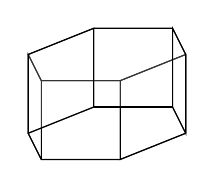
\begin{tikzpicture}[ rotate around z=0, rotate around x=90]
\coordinate (p0) at (1, 0, 0);
\coordinate (p1) at (0.5,0.866,0);
\coordinate (p2) at (-0.5, 0.866, 0);
\coordinate (p3) at (-1, 0, 0);
\coordinate (p4) at (-0.5,-0.866,0);
\coordinate (p5) at (0.5,-0.866,0);

\filldraw[fill opacity=0.2, fill=white] (p0)\foreach
	\x in {1, 2, 3, 4, 5, 0} {
	-- (p\x)
};

\coordinate (q0) at (1, 0, 1);
\coordinate (q1) at (0.5,0.866,1);
\coordinate (q2) at (-0.5, 0.866, 1);
\coordinate (q3) at (-1, 0, 1);
\coordinate (q4) at (-0.5,-0.866,1);
\coordinate (q5) at (0.5,-0.866,1);

\filldraw[fill opacity=0.2, fill=white] (q0)\foreach
	\x in {1, 2, 3, 4, 5, 0} {
	-- (q\x)
};
\foreach
	\x in {0, 1, 2, 3, 4, 5} {
	\pgfmathsetmacro{\y}{ \intcalcMod{\x + 1}{6}};
	\filldraw[fill opacity=0.2, fill=white] (q\x) -- (q\y) -- (p\y) -- (p\x) -- (q\x);
};

\end{tikzpicture}

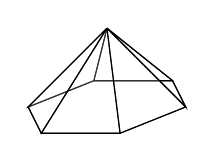
\begin{tikzpicture}[rotate around x=-90]
\coordinate (p0) at (1, 0, 0);
\coordinate (p1) at (0.5,0.866,0);
\coordinate (p2) at (-0.5, 0.866, 0);
\coordinate (p3) at (-1, 0, 0);
\coordinate (p4) at (-0.5,-0.866,0);
\coordinate (p5) at (0.5,-0.866,0);

\filldraw[fill opacity=0.2, fill=white] (p0)\foreach
	\x in {1, 2, 3, 4, 5, 0} {
	-- (p\x)
};

\coordinate (q0) at (0, 0, 1);
\coordinate (q1) at (0, 0, 1);
\coordinate (q2) at (0, 0, 1);
\coordinate (q3) at (0, 0, 1);
\coordinate (q4) at (0, 0, 1);
\coordinate (q5) at (0, 0, 1);

\filldraw[fill opacity=0.2, fill=white] (q0)\foreach
	\x in {1, 2, 3, 4, 5, 0} {
	-- (q\x)
};
\foreach
	\x in {0, 1, 2, 3, 4, 5} {
	\pgfmathsetmacro{\y}{ \intcalcMod{\x + 1}{6}};
	\filldraw[fill opacity=0.2, fill=white] (q\x) -- (q\y) -- (p\y) -- (p\x) -- (q\x);
};

\end{tikzpicture}

\section{Skew group algebra S\#G indecomposable projectives}
This section is largely based on the book by \cite{CMR}. This section will use definitions and theorems from representation theory as taught in the courses MA3203 - Ring Theory and MA3204 - homological algebra. Since I do not assume knowledge of this I have created appendix \ref{appendix}. I will try to use footnotes to indicate where such theorems are used.

\begin{defin}
If $G$ is a subgroup of $GL_n(\C)$, we can extend the group action of $G$ on $\C^n$ to $\C\llbracket x_1, \cdots, x_n\rrbracket$. More explicitly $G$ acts on $x_i$ as it would the $i$th basis vector of $\C^n$, and acts on products and sums by acting on each component separately. We then define the \underline{skew group algebra $\C \llbracket x_1, \cdots, x_n \rrbracket \# G$} to be the algebra generated by elements of the form $f \cdot g$ with $f \in \C\llbracket x_1, \cdots, x_n\rrbracket$ and $g \in G$, and we define the multiplication by
$$ (f_1 \cdot g_1) \cdot (f_2 \cdot g_2) = (f_1 \cdot f_2^{g_1}) \cdot (g_1 \cdot g_2) $$
Where $f^g$ denotes the image of $f$ under the action of $g$.
\end{defin}

The skew group algebra is also sometimes called the twisted algebra, because the multiplication is "twisted" by the action of $G$.

\begin{lemma}
\label{lem:S proj => SG proj}
Let $S = \C\llbracket x, y \rrbracket$. An $S\#G$-module is projective\footnote{The definition of projective can be found in \cref{def:projective} on page \pageref{def:projective}.} if and only if it is projective as an $S$-module.

\begin{proof}
Only-ifity follows from $S\#G$ being a free $S$-module, it is isomorphic to $\bigoplus_{g \in G} S$. Thus we need only show ifity.

First we need to see that an $S\#G$-linear map is just an $S$-linear map, $f: M \to N$ between $S\#G$-modules, such that $f(g(m))=g(f(m))$ for all $g \in G$ and all $m \in M$. Equivalently $f(m) = g(f(g^{-1}(m)))$. This allows us to define a group action on $S$-linear maps by $f^g(m) = g(f(g^{-1}(m)))$. Then we just need to show $$ \Hom_{S\#G}(M,N) = \Hom_S(M,N)^G.$$
Clearly if $f$ is $S\#G$-linear then it's in $\Hom_S(M,N)^G$. To see the other inclusion, let $f$ be an $S$-linear map that is fixed under $G$. Then $f(s\cdot g m) = s f(g m) = s\cdot g(f(g^{-1} g m)) = s \cdot g f(m) $, and hence $f$ is $S\#G$-linear.

Nextly we want to show that $-^G$ is an exact functor\footnote{The definition of an exact functor can be found in \cref{def:exact_functor} on page \pageref{def:exact_functor}.}. If $K$ is the kernel of a map $f: M \to N$, then the kernel of the induced map $f^G : M^G \to N^G$ is of course just $K \cap M^G$ which equals $K^G$. Assume $f$ is epi and let $n \in N^G$. Consider a preimage $m$ such that $f(m)=n$. Let $\theta = \frac{1}{|G|}\sum_{g \in G} g(m)$. Then $\theta$ is in $M^G$ and $f(\theta) = \frac{1}{|G|}\sum_{g \in G} g(f(m)) = \frac{1}{|G|}\sum_{g \in G} n = n$.

Recall that a module being projective is equivalent to its covariant $\Hom$-functor being exact. So if $P$ is projective as an $S$-module then $\Hom_S(P, -)$ is exact. Using our above result we get $\Hom_S(P, -)^G = \Hom_{S\#G}(P, -)$ is exact and our lemma follows.
\end{proof}
\end{lemma}

\begin{lemma}
\label{lem:radical small}
Let $S$ be the complex power series ring in $n$ variables, and $\mathfrak{m} = \langle x_i \rangle_{i=1}^n$ the radical of $S$. Then for any free $S$-module $N$, $\mathfrak{m}N$ is \underline{small} in $N$. That is if $X$ is  a submodule of $N$ such that $X + \mathfrak{m}N = N$, then $X = N$.

\begin{proof}
Let $N$ be the free module $S^{(I)} := \bigoplus\limits_{i \in I} S_i$, where $S_i \cong S$. Assume that $X$ is a submodule such that $X + \mathfrak{m}N = N$. We denote by $1_i$ the elements that is 1 at index $i$ and 0 elsewhere. Since $\{ 1_i \}$ generate $N$, it is enough to show that $X$ contains all of them. Since $X + \mathfrak{m}N = N$, we know that there is an $m_i \in \mathfrak{m}N$ and an $x_i \in X$ such that $x_i + m_i = 1_i$. Then we have that $x_i = 1_i - m_i$. Since the power series at index $i$ of $x_i$ has constant coefficient 1 it is invertible. If we multiply $x_i$ by its inverse we get $\tilde{x}_i$ which is 1 at index $i$ and some element of $\mathfrak{m}$ at index $j \neq i$, say $m_{ij}$. Then $\tilde{x}_i - \sum\limits_{j \neq i} m_{ij}\tilde{x}_j$ has a unit in index $i$ and 0 at all other indices. Thus $X$ contains $1_i$ for all $i$, and $X = N$.
\end{proof}
\end{lemma}

\begin{theorem}
\label{thm:indec_proj_SG=indec_CG}
Let $S = \C\llbracket x, y \rrbracket$ and let $\mathfrak{m} = \langle x, y \rangle_S$ be the radical of $S$. Then there are bijections between the indecomposable\footnote{The definition of indecomposable can be found in \cref{def:indecomposable} on page \pageref{def:indecomposable}.} finitely generated projective $S\#G$-modules and the indecomposable $\C G$-modules given by
\\
\\
\begin{tikzcd}
\left\lbrace \begin{matrix}
\text{indecomposable projective}\\
S\#G\text{-modules}
\end{matrix} \right\rbrace \ar[r, ->]
& 
\left\lbrace \begin{matrix}
\text{indecomposable}\\
\C G\text{-modules}
\end{matrix} \right\rbrace\\
\mathcal{F}: P \arrow[mapsto]{r} & P/\mathfrak{m}P\\
\mathcal{G}: S \otimes_\C W & W \arrow[mapsto]{l}
\end{tikzcd}

Where the $S\#G$-module structure on $S \otimes_\C W$ is given by $(s \cdot g) \cdot f \otimes v = sf^g \otimes v^g$.

\begin{proof}
First we should show that $S \otimes_\C W$ is an indecomposable projective $S\#G$-module and that $P/\mathfrak{m}P$ is in fact an indecomposable $\C G$-module. Since $S \otimes_\C W$ is a free $S$-module it follows from \cref{lem:S proj => SG proj} that it is projective. To see that it is indecomposable we will first study it as an $S$-module and exploit the fact that $\Hom_{S\#G}(M,N) \subseteq \Hom_S(M,N)$. 

Using \cref{lem:radical small} we get that $\mathfrak{m}S \otimes_\C W$ is small in $S\otimes_\C W$. This means that we get that 
\begin{align*}
\frac{S \otimes_\C W}{\mathfrak{m}S \otimes_\C W} \cong S/\mathfrak{m} \otimes_\C W \cong \C \otimes_\C W \cong W
\end{align*}
and therefore $S \otimes_\C W \to W$ is a projective cover\footnote{The definition of projective cover can be found in \cref{def:projective_cover} on page \pageref{def:projective_cover}.} of $W$ as $S$-modules. Further since the projection $S \otimes_\C W \to W$ is $S\#G$-linear we have that $S \otimes_\C W$ is the projective cover of $W$ also as $S\#G$-modules. Assume for the sake of contradiction that $S \otimes_\C W$ decomposes as $M \oplus N$ for non-zero $M$ and $N$. Then $W$ would equal $M/\mathfrak{m}M \oplus N/\mathfrak{m}N$ as an $S\#G/ \langle \mathfrak{m} \rangle$-module. Since $S\#G/ \langle \mathfrak{m} \rangle \cong \C G$ and $W$ is indecomposable we must have that either $M/\mathfrak{m}M$ or $N/\mathfrak{m}N$ is 0. This then gives a contradiction because $\mathfrak{m}M$ and $\mathfrak{m}N$ are small in $M$ and $N$. Hence we must have that $S \otimes_\C W$ is indecomposable.

It's clear that $P/\mathfrak{m}P$ is a $\C G$-module, because $\C G$ is a subring of $S\#G$. To see that it's indecomposable we will use a similar argument as above. Assume $P/\mathfrak{m}P$ decomposes as $V \oplus W$. Then both $P$ and $S\otimes_\C V \oplus S \otimes_\C W$ are projective covers of $P/\mathfrak{m}P = V\oplus W$ we get induced $S\#G$-linear epimorphisms between them.

\begin{center}
\begin{tikzcd}
& S \otimes_\C P/\mathfrak{m}P \arrow[twoheadrightarrow]{d} \arrow[dashed, two heads, bend right=20]{dl}\\
P \arrow[->>]{r} \arrow[dashed, two heads, bend right=5]{ur} & P/\mathfrak{m}P
\end{tikzcd}
\end{center}

Now we use the fact that $P$ is finitely generated. Since there can only be an epimorphism from a module with more or equal amount of generators, $P$ and $S\otimes_\C \mathfrak{m}P$ must have the same amount of generators and the induced maps are in fact isomorphisms of $S$-modules. Since the maps are also $S\#G$-linear we have that $P$ decomposes as $S\otimes_\C V \oplus S \otimes_\C W$. Then since $P$ is indecomposable we must have that either $S \otimes_\C V$ or $S\otimes_\C W$ is 0. That means that either $V$ or $W$ is 0, and we have shown that $P/\mathfrak{m}P$ is an indecomposable $\C G$-module.

To see that the given maps are bijections we will show that they are mutual inverses. First to see that $\mathcal{F}(\mathcal{G}(W)) \cong W$ we simply look at the definition
\begin{equation*}
\begin{split}
\frac{S \otimes_\C W}{\mathfrak{m}S \otimes_\C W} \cong S/\mathfrak{m} \otimes_\C W \cong \C \otimes_\C W \cong W
\end{split}
\end{equation*}

Next we consider $\mathcal{G}(\mathcal{F}(P)) = S \otimes_\C P/\mathfrak{m}P$. We have already seen that the induced map
\begin{center}
\begin{tikzcd}
& S \otimes_\C P/\mathfrak{m}P \arrow[twoheadrightarrow]{d} \arrow[dashrightarrow]{dl}\\
P \arrow[->>]{r} & P/\mathfrak{m}P
\end{tikzcd}
\end{center}
is an isomorphism, and thus $P \cong \mathcal{G}(\mathcal{F}(P))$.
\end{proof}

\end{theorem}

\subsection{The Gabriel quiver}
Now that we have seen that the indecomposable $\C G$-modules and the indecomposable finitely generated projective $S\#G$-modules are in correspondence we will construct the quiver that corresponds to the McKay quiver.

\begin{defin}
For a skew group algebra $S\#G$ we define its \underline{Gabriel quiver} to be the quiver with vertices as the indecomposable projective modules of $S\#G$. The arrows are given by taking the minimal projective resolution\footnote{The definition of a minimal projective resolution can be found in \cref{def:projective_resolution} on page \pageref{def:projective_resolution}.} of $P/\mathfrak{m}P$, where $\mathfrak{m}$ is as defined above. If the minimal projective resolution of $P/\mathfrak{m}P$ is given by
\begin{center}
\begin{tikzcd}
\cdots \arrow{r} & Q_1 \arrow{r} & Q_0 \arrow{r} & 0
\end{tikzcd}
\end{center}
We say there is an arrow from $P$ to $P'$, if $P'$ appears as a direct summand of $Q_1$.
\end{defin}

\begin{defin}
Let $V$ be a vector space. We then define the exterior algebra $\bigwedge V$ as the associative unital graded algebra such that the multiplication is bilinear and satisfies $x \wedge y = -y \wedge x$ for any $x$ and $y$ in $V$.
\end{defin}
Some key properties of the exterior algebra is that $x \wedge x = 0$, and more generally that $x_1 \wedge \cdots \wedge x_p = 0$ whenever $\{x_i\}_{i=1}^p$ are linearly dependent.

The $p$th exterior power of $V$, denoted $\bigwedge\limits^p V$ is the vector space of all elements that are the product of $p$ vectors in $V$. If $\{ x_i \}_{i=1}^n$ is a basis for $V$, then $x_{i_1} \wedge \cdots \wedge x_{i_p}$ where $i_1 < i_2 < \cdots < i_p$ and $1 \leq i_j \leq n$ forms a basis for $\bigwedge\limits^p V$, thus it is ${n \choose p}$-dimensional. 

\begin{prop}
If $S$ is the ring of formal power series over $\C$ in $n$ variables, and $G$ is a finite group acting on $S$, let $V=\mathfrak{m}/\mathfrak{m}^2$. Then the minimal projective resolution of $\C \cong S/\mathfrak{m}$ as an $S$-module is given by
\begin{center}
\begin{tikzcd}
0  \arrow{r} & S \otimes_\C \bigwedge\limits^n V  \arrow{r}{\partial_n} & \cdots \arrow{r}{\partial_2} & S \otimes_\C \bigwedge\limits^{1} V \arrow{r}{\partial_1} & S \arrow{r} & 0
\end{tikzcd}
\end{center}
Where $\partial_p$ is the $S\#G$-linear map defined by
\begin{align*}
\partial_p(s \otimes x_{i_1} \wedge x_{i_2} \wedge \cdots \wedge x_{i_p}) = \sum_{j=1}^{p} (-1)^{j+1} sx_{i_j} \otimes x_{i_1} \wedge \cdots \wedge \hat{x}_{i_{j}} \wedge \cdots \wedge x_{i_{p}}
\end{align*}
Where $x_{i_1} \wedge x_{i_2} \wedge \cdots \wedge x_{i_p}$ is one of the standard basis vectors for $\bigwedge\limits^n V$, namely $i_1 < i_2 < \cdots < i_p$, and  $\hat{x}_j$ means that $x_j$ is omitted.

\begin{proof}
First we should show that this is a projective resolution of $\C$. In fact the complex described above is the Koszul complex of the regular sequence\footnote{Regular sequences are defined on page \pageref{def:regular_seq} in \cref{def:regular_seq}.} $(x_i)_{i=1}^n$. The Koszul complex of a regular sequence is a projective resolution of the ring modulo the ideal generated by the regular sequence \cite[\href{https://stacks.math.columbia.edu/tag/062F}{Tag 062F}]{stacks-project}, which in this case equals $S/\langle x_i \rangle_{i=1}^n = \C$.

Secondly we want to show that the resolution is minimal. To do this it is enough to show that for each $k \geq 1$, $\partial_k$ is a projective cover of its image, and that $S \to \C$ is a projective cover of $\C$. In other words we have to show that the kernels of the maps are small. Since $\Image \partial_{k+1} = \Ker \partial_k$ and $\Image \partial_{k+1} \subseteq \mathfrak{m} \otimes_\C \bigwedge\limits^{k+1}V$ it follows from \cref{lem:radical small} that the resolution is minimal.
\end{proof}
\end{prop}

Since $V = \mathfrak{m}/\mathfrak{m}^2 = \langle x_1, x_2, \cdots, x_n \rangle_\C$ is exactly the canonical representation of $G$ the relationship between the McKay quiver and the Gabriel quiver should be apparent. Now we move to the next theorem for a formal argument.

\begin{theorem}
If $S$ is the complex power series ring in $n$ variables and $G$ is a finite subgroup of $GL_n(\C)$, then the McKay quiver of $G$ and the Gabriel quiver of $S\#G$ are isomorphic.
\begin{proof}
We have already seen in \cref{thm:indec_proj_SG=indec_CG} that they have the same vertices, namely if $V_i$ are the irreducible representations of $G$, then $S \otimes_\C V_i$ are the indecomposable projectives of $S\#G$. To see that they have the same arrows consider as above the minimal resolution of $\C$:
\begin{center}
\begin{tikzcd}
0  \arrow{r} & S \otimes_\C \bigwedge\limits^n V  \arrow{r}{\partial_n} & \cdots \arrow{r}{\partial_2} & S \otimes_\C \bigwedge\limits^{1} V \arrow{r}{\partial_1} & S \arrow{r} & 0.
\end{tikzcd}
\end{center}
If we tensor with $V_i$ on the right we will get a minimal resolution of $V_i$:
\begin{center}
\begin{tikzcd}
\cdots \arrow{r}{\partial_2 \otimes_\C V_i} & S \otimes_\C \bigwedge\limits^{1} V \otimes_\C V_i \arrow{r}{\partial_1 \otimes_\C V_i} & S \otimes_\C V_i \arrow{r} & 0.
\end{tikzcd}
\end{center}
From here, since $\bigwedge\limits^{1} V = V$, we see that $P_j = S \otimes_\C V_j$ appears as a direct summand of $S \otimes_\C V \otimes_\C V_i$ exactly when $V_j$ appears as a direct summand of $V \otimes_\C V_i$.
\end{proof}
\end{theorem}

\section{The endomorphism ring of $S$ as an $S^G$-module}
This section is largely based on the article by \cite{IyTa} and the book by \cite{CMR}.

In this section we will show that $S\#G$ is isomorphic to $\End_R(S)$ as rings, where $S$ is the complex power series ring in 2 variables, $G$ is a finite subgroup of $SL_2(\C)$, and $R = S^G$ is the fixed ring of $S$ by $G$. This will be the longest proof of this thesis and I have therefore decided to split it up into several steps. The proof will be done by constructing an explicit isomorphism.
\begin{center}
\begin{tikzcd}
S\#G \ar[r] & \End_R(S)\\
s \cdot g \ar[r, mapsto] & (t \mapsto s \cdot t^g)
\end{tikzcd}
\end{center}
We can easily show that this is an injective ring-homomorphism. The meat of the proof is to consider the map as a morphism of $R$-modules, and then using ramification theory to show that it is an epimorphism. We will show in \cref{thm:unramified_pseudoreflections} that for every height one prime ideal $\mathfrak{p}$ of $S$ if we localize\footnote{Prime ideals and localization will be defined later in \cref{def:prime_ideal} and \cref{def:localization}.} at $\mathfrak{p}$ we get a so-called unramified extension of rings
\begin{center}
\begin{tikzcd}
R_{\mathfrak{p} \cap R} \ar[hook, r] & S_\mathfrak{p}.
\end{tikzcd}
\end{center}
Then \cref{thm:unramified_implies_seperable} will give use that the extension is separable. That is, we have a split exact sequence
\begin{center}
\begin{tikzcd}
I \ar[hook, r] & S_\mathfrak{p} \otimes_{R_{\mathfrak{p} \cap R}} S_\mathfrak{p} \ar[two heads, r]{}{\mu} & S_\mathfrak{p}
\end{tikzcd}
\end{center}
where $\mu$ is the multiplication map and $I$ is the kernel of $\mu$. Now writing $\mathfrak{q} = \mathfrak{p} \cap R$, and $S_\mathfrak{q}$ for $R_\mathfrak{q} \otimes_R S$, what we really want is a split exact sequence
\begin{center}
\begin{tikzcd}
I \ar[hook, r] & S_\mathfrak{q} \otimes_{R_{\mathfrak{q}}} S_\mathfrak{q} \ar[two heads, r]{}{\mu} & S_\mathfrak{q}
\end{tikzcd}
\end{center}
We will use this splitting in \cref{thm:separable_implies_ringiso} to construct an inverse for $S_\mathfrak{q}\#G \to \End_{R_{\mathfrak{q}}}(S_\mathfrak{q})$. Finally we will show that since we get an isomorphism whenever we localize at a height one prime ideal, \cref{lem:height_one_iso} and \cref{thm:skew_group_algerba_equals_endomorphsim_ring} will give us that the map is an isomorphism.

Let us first begin with some definitions
\begin{defin}
If $A$ is a local ring with residual field $k$ we define the \underline{depth} of a module, $M$, to be the minimal $n$ such that $\Ext^n_A(k, M)$ is non-zero\footnote{The extension group is defined in \cref{def:Ext} on page \pageref{def:Ext}.}. We write $\depth_A(M)$ for this or simply $\depth(M)$ when which ring we are using is clear.
\end{defin}

\begin{defin}
\label{def:regular_seq}
If $R$ is a commutative ring and $M$ is an $R$-module, an \underline{$R$-regular sequence on $M$} is a sequence of elements of $R$, $r_1, r_2, \cdots r_n$ such that $M/\langle r_1, \cdots, r_i \rangle M$ is non-zero and multiplication by $r_i$ is injective on $M/\langle r_1, \cdots, r_{i-1} \rangle M$.
\end{defin}

\begin{prop}
For a module over a local ring all maximal regular sequences have the same length. That length is the depth of the module.
\begin{proof}
The proof is omitted here, but can be found in \cite[\href{https://stacks.math.columbia.edu/tag/00LW}{Tag 00LW}]{stacks-project} and \cite[\href{https://stacks.math.columbia.edu/tag/090R}{Tag 090R}]{stacks-project}.
\end{proof}
\end{prop}

\begin{defin}
\label{def:prime_ideal}
If $R$ is a ring, we say that $\mathfrak{p}$ is  a \underline{prime ideal} in $R$ if
\begin{enumerate}
\item $\mathfrak{p}$ is a proper ideal of $R$.
\item For any two elements $a,b \in R$ such that $ab \in \mathfrak{p}$ we must have that either $a$ is in $\mathfrak{p}$ or $b$ is.
\end{enumerate}
The \underline{height} of $\mathfrak{p}$ is the length of the longest chain of prime ideals contained in $\mathfrak{p}$:
\begin{align*}
\mathfrak{p}_0 \subset \mathfrak{p}_1 \subset \cdots \subset \mathfrak{p}_n = \mathfrak{p}.
\end{align*}
\end{defin}

\begin{defin}
\label{def:localization}
Let $R$ be a commutative ring, $M$ an $R$-module, and $\mathfrak{p} \subset R$ a prime ideal of $R$. Then we define the \underline{loclization of $M$ at $\mathfrak{p}$}, written as $M_\mathfrak{p}$, to be the set of formal fractions $\frac{m}{r}$ with $m$ in $M$ and $r$ in $R \setminus \mathfrak{p}$. Two such fractions $\frac{m}{r}$ and $\frac{n}{s}$ are considered the same if there is an element $t \in R \setminus \mathfrak{p}$ such that $t(sm - rn) = 0$.

Note that if we localize $R$ at $\mathfrak{p}$ we get an $R$-algebra with the multiplication $\frac{r}{s} \cdot \frac{r'}{s'} = \frac{rr'}{ss'}$, as you would expect. In fact it's enough to understand $R_\mathfrak{p}$ because $M_\mathfrak{p} = R_\mathfrak{p} \otimes_R M$.
\end{defin}

\begin{defin}
Let $A$ and $B$ be two local commutative rings with maximal ideal $\mathfrak{n}$ and $\mathfrak{m}$ respectively, and let
\begin{tikzcd}
A \ar[hook, r] & B
\end{tikzcd}
be an extension of rings. We say that the extension is \underline{unramified} if the following conditions hold:
\begin{itemize}
\item $B$ is a finitely generated $A$-module.
\item \begin{tikzcd}
A/\mathfrak{n} \ar[hook, r] & B/\mathfrak{m}
\end{tikzcd}
is a separable field extension.
\item $\mathfrak{n}B = \mathfrak{m}$
\end{itemize}
If the two first conditions are met, and there is a positive integer $e$ such that $\mathfrak{n} B = \mathfrak{m}^e B$, we say the extension has \underline{ramification index} $e$ when $e$ is the smallest such number. Note that being unramified is then equivalent to having ramification index 1.
\end{defin}

In order to show that unramified implies separable we must first take a small detour.

\begin{defin}
Let $A \to B$ be an extension of rings. We then define the \underline{derivation module} $\Omega_{B | A}$ as the $B$-module with formal generators $db$ for all $b \in B$ and with the following relations:
\begin{itemize}
\item[$A$-linearity:] $d(ab + a'b') = adb + a'db'$ for all $a, a' \in A$ and $b, b' \in B$.
\item[Leibniz rule:] $d(bc) = bdc + cdb$ for all $b,c \in B$.
\end{itemize}
\end{defin}
Note that for any polynomial expression $f(b)$ we have that $df(b) = f'(b)db$ where $f'$ is the formal derivative of $f$. Now we will show how the derivation module make a link between unramified extensions and the splitting of our sequence.

\begin{prop}
Let $A \to B$ be an unramified extension of local rings. Then $\Omega_{B|A}$ is $0$.

\begin{proof}
Keeping with the notation above we let $\mathfrak{n}$ be the maximal ideal of $A$ and $\mathfrak{m}$ the maximal ideal of $B$. Furthermore let $l$ denote $B/\mathfrak{m}$ and $k$ denote $A/\mathfrak{n}$. Then we claim there is an exact sequence
\begin{center}
\begin{tikzcd}
\mathfrak{m}/\mathfrak{m}^2 \ar[r]{}{\alpha} & \Omega_{B|A} \otimes_B B/\mathfrak{m} \ar[r] & \Omega_{l|A} \ar[r] & 0
\end{tikzcd}
\end{center}
where $\alpha(\overline{m}) = d_{B|A}m \otimes 1$ for any $m$ in $\mathfrak{m}$. Let's first show that $\alpha$ is well defined. Let $m_1 \cdot m_2$ be in $\mathfrak{m}^2$. Then we need to show that $\alpha(\overline{m_1 \cdot m_2})$ is 0.
\begin{align*}
\alpha(\overline{m_1 \cdot m_2}) &= d_{B|A}(m_1 \cdot m_2) \otimes 1 =\\
m_1 d_{B|A}m_2 \otimes 1 &+ m_2d_{B|A}m_1 \otimes 1 =\\
d_{B|A}m_2 \otimes (m_1 \cdot 1) &+ d_{B|A}m_1 \otimes (m_2 \cdot 1)
\end{align*}
Since $l = B/\mathfrak{m}$ we have that $m_1 \cdot 1$ and $m_2 \cdot 1$ is 0 in $l$, thus the right hand side is 0, and $\alpha$ is well defined.

The map $\Omega_{B|A} \otimes_B B/\mathfrak{m} \to \Omega_{l|A}$ is just the natural projection sending $db \otimes 1$ to $d\overline{b}$, where $\overline{b}$ is the projection of $b$ onto $l$. We want to show that this is the cokernel of $\alpha$. The kernel of $\Omega_{B|A} \otimes_B B/\mathfrak{m} \to \Omega_{l|A}$ is generated by $dm \otimes 1$ for $m \in \mathfrak{m}$, but this is exactly the image of $\alpha$, thus the sequence is exact.

Nextly we want to show that $\Omega_{l|A} = 0$. Since $\mathfrak{n} \subseteq \mathfrak{m}$ and $l$ is annihilated by $\mathfrak{m}$ we have that $\Omega_{l|A} = \Omega_{l|k}$. Let $x$ be an element of $l$, and let $p$ be its irreducible polynomial over $k$. Now we want to use the fact that $k \subset l$ is a separable field extension. Remember that $k \subset l$ being separable means that the formal derivative of $p$ is non-zero. Now we have that
\begin{align*}
0 = d(p(x)) = p'(x)dx.
\end{align*}
Since $p'$ is a non-zero polynomial of lower degree than $p$, and $p$ is the smallest polynomial with root $x$, we must have that $p'(x)$ is non-zero. This implies that $dx=0$, and since this holds for all $x$ it must be that $\Omega_{l|k}=0$.

Since $\Omega_{l|k}=0$ we have that $\alpha$ is surjective. We will now use that since $A \to B$ is unramified $\mathfrak{n}B = \mathfrak{m}$. More specifically the map $\beta: \mathfrak{n}/\mathfrak{n}^2 \otimes_A B \to \mathfrak{m}/\mathfrak{m}^2$ is surjective. Since both $\alpha$ and $\beta$ are surjective we have that $\alpha\beta$ is also surjective, but
\begin{align*}
\alpha\beta(\overline{n} \otimes b) = \alpha(\overline{nb}) = d(nb) \otimes 1 = ndb \otimes 1 = db \otimes n \cdot 1 = 0
\end{align*}
for all $n \in \mathfrak{n}$ and $b \in B$. Thus the only conclusion is that $\Omega_{B|A} \otimes_B l = 0$.

Since $\Omega_{B|A} \otimes_B l = \Omega_{B|A} \otimes_B B/\mathfrak{m} = \Omega_{B|A}/\mathfrak{m}\Omega_{B|A}$ it follows from Nakayama's lemma \cite[\href{https://stacks.math.columbia.edu/tag/07RC}{Tag 07RC}]{stacks-project} that $\Omega_{B|A}=0$.
\end{proof}
\end{prop}

\begin{theorem}
\label{thm:unramified_implies_seperable}
Let $A \to B$ be an unramified extension of local rings. Then the sequence
\begin{center}
\begin{tikzcd}
0 \ar[r] & I \ar[r] & B \otimes_A B \ar{r}{\mu} & B \ar[r] & 0
\end{tikzcd}
\end{center}
splits as a short exact sequence of $B\otimes_AB$-modules. Here $\mu$ is given by $\mu(b \otimes b') = bb'$, and the $B \otimes_A B$-module structure on $B$ is given by $b \otimes b' \cdot b'' = bb'b''$, and $I = \Ker \mu$. We say that the extension is separable

\begin{proof}
Firstly note that $I$ is generated by elements on the form $b \otimes 1 - 1 \otimes b$, and that since $B$ is finitely generated as an $A$-module, $I$ is finitely generated.

Next we want to show that $I/I^2 = \Omega_{B|A}$, which we have already seen equals 0. Since $\Omega_{B|A}$ is a $B$-module we need a $B$-module structure on $I/I^2$. Since $(b \otimes 1)i - (1\otimes b)i$ is in $I^2$ for $i \in I$, we have that $(b \otimes 1)i = (1 \otimes b)i \mod I^2$. Then $I/I^2$ is generated by $(c \otimes 1 - 1 \otimes c)$ as a $B$-module with the $B$-module action given by $b \cdot i := (1 \otimes b)i$.

Now to see that $I/I^2 = \Omega_{B|A}$ we will show that the relations on $(b \otimes 1 - 1 \otimes b)$ in $I/I^2$ are exactly the same as those for $db$ in $\Omega_{B|A}$, thus that $(db \mapsto (b \otimes 1 - 1 \otimes b))$ is an isomorphism.

$A$-linearity follows from the fact that we are tensoring over $A$, that is
\begin{align*}
(ab \otimes 1 - 1 \otimes ab) &= (b \otimes a - 1 \otimes ab) =\\
(1 \otimes a)(b \otimes 1 - 1 \otimes b) &= a \cdot
(b \otimes 1 - 1 \otimes b)
\end{align*}

The Leibniz rule $dbc - bdc - cdb = 0$ follows from a similar computation.
\begin{align*}
& \;(b \otimes 1 - 1 \otimes b)(c \otimes 1 - 1 \otimes c) \\
=&\; bc \otimes 1 - b \otimes c - c \otimes b + 1 \otimes bc \\
=&\; (bc \otimes 1 - 1 \otimes bc) - (c \otimes b - 1 \otimes bc) - (b \otimes c - 1 \otimes bc)\\
=&\; (bc \otimes 1 - 1 \otimes bc) - (1 \otimes b)(c \otimes 1 - 1 \otimes c) - (1 \otimes c)(b \otimes 1 - 1 \otimes b)\\
\end{align*}
and we see that $(bc \otimes 1 - 1 \otimes bc) - b \cdot (c \otimes 1 - 1 \otimes c) - c \cdot (b \otimes 1 - 1 \otimes b)$ generates $I^2$.

Now that we have shown that $I/I^2 = \Omega_{B|A} = 0$, or rather that $I = I^2$. Nakayama's lemma gives that there is an $i \in I$ such that $ji = j$ for all $j \in I$. Then we can define the splitting map $B \otimes_A B \to I$ by $b \otimes b' \mapsto b \otimes b' \cdot i$. Thus the sequence
\begin{center}
\begin{tikzcd}
0 \ar[r] & I \ar[r] & B \otimes_A B \ar{r}{\mu} & B \ar[r] & 0
\end{tikzcd}
\end{center}
splits.
\end{proof}
\end{theorem}

\begin{theorem}
\label{thm:separable_implies_ringiso}
Let $B$ be a local $k$-algebra domain, and $G$ a finite subgroup of $\Aut_k(B)$ with order relatively prime to the characteristic of $k$, and denote by $A$ the fixed ring $B^G$. If the short exact sequence
\begin{center}
\begin{tikzcd}
0 \ar[r] & I \ar[r] & B \otimes_A B \ar{r}{\mu} & B \ar[r] & 0
\end{tikzcd}
\end{center}
splits, then the map
\begin{center}
\begin{tikzcd}
B\#G \ar[r]{}{\gamma} & \End_A(B)\\
b \cdot g \ar[mapsto, r] & (a \mapsto b \cdot a^g)
\end{tikzcd}
\end{center}
is an isomorphism of $A$-modules, and isomorphism of rings.

\begin{proof}
First in order to see that the map is injective, assume $b \cdot g$ and $b' \cdot g'$ map to the same endomorphism. Then $b \cdot t^g = b' \cdot t^{g'}$ for all $t \in B$. Choosing $t=1$ we see that $b = b'$. Then since $B$ is a domain this means that $t^g = t^{g'}$ for all $t$, that is to say $g = g'$.

To see that the map is surjective we will construct a splitting. The splitting will be constructed using the following diagram:
\begin{center}
\begin{tikzcd}
B\#G \ar[r]{}{\gamma} & \End_A(B) \ar[d]{}{f \mapsto f \otimes \rho}\\
B \otimes_A B\#G \ar{u}{\tilde{\mu}} & \Hom_B(B \otimes_A B, B \otimes_A B\#G) \ar[l]{}{ev_\epsilon}
\end{tikzcd}
\end{center}
where $\rho$ is the modified Reinolds-operator
\begin{center}
\begin{tikzcd}
\rho(b) = \sum\limits_{g \in G} b^g \cdot g.
\end{tikzcd}
\end{center}
Since we assumed the extension is unramified we have that
\begin{center}
\begin{tikzcd}
0 \ar[r] & I  \ar[r]{}{\iota} & B \otimes_A B \ar[r]{}{\mu} \ar[l, dotted, bend left = 30]{}{\psi} & B \ar[r] & 0
\end{tikzcd}
\end{center}
splits. As indicated we denote the left splitting by $\psi$. Then let $\epsilon = 1 \otimes 1 - \iota\psi(1 \otimes 1)$ in $B \otimes_A B$. Then $\mu(\epsilon) = 1$, and $(b \otimes 1 - 1 \otimes b)\epsilon = 0$. Then we define the evaluation map at $\epsilon$ by
\begin{center}
\begin{tikzcd}
ev_\epsilon: & \Hom_B(B \otimes_A B, B \otimes_A B\#G) \ar[r] & B \otimes_A B\#G\\
& f \ar[r, mapsto] & f(\epsilon)
\end{tikzcd}
\end{center}
Lastly $\tilde{\mu}: B \otimes_A B\#G \to B\#G$ is simply the map $b \otimes c \cdot g \mapsto bc \cdot g$. We have now defined all the maps in the square
\begin{center}
\begin{tikzcd}
B\#G \ar[r]{}{\gamma} & \End_A(B) \ar[d]{}{f \mapsto f \otimes \rho}\\
B \otimes_A B\#G \ar{u}{\tilde{\mu}} & \Hom_B(B \otimes_A B, B \otimes_A B\#G) \ar[l]{}{ev_\epsilon}
\end{tikzcd}
\end{center}
Now we want to show that the composition of the three bottom maps forms a splitting. That is for any $f \in \End_A(B)$ we have that $\gamma(\tilde{\mu}(ev_\epsilon(f \otimes \rho))) = f$.

Write $\epsilon = \sum\limits_i x_i \otimes y_i$. Then we claim that
\begin{align*}
\sum_i x_i y_i^g = \begin{cases}
1 & g = 1_G\\
0 & \text{otherwise}
\end{cases}
\end{align*}
We know that
\begin{align*}
(b \otimes 1)\sum_i x_i \otimes y_i = (1 \otimes b)\sum_i x_i \otimes y_i
\end{align*}
holds for all $b$. Then applying the map $1 \otimes g$ on both sides we get
\begin{align*}
\sum_i bx_i \otimes y_i^g = \sum_i x_i \otimes b^gy_i^g
\end{align*}
Then by applying $\mu$ we get
\begin{align*}
b\sum_i x_i y_i^g = b^g\sum_i x_i  y_i^g
\end{align*}
Then since $B$ is a domain we get that either $b = b^g$ or $\sum_i x_i  y_i^g = 0$. If we assume that $\sum_i x_i  y_i^g \neq 0$ then we must have that $b = b^g$ for all $b \in B$ and we then get that $g = 1_G$. Then since
\begin{align*}
\sum_i x_i  y_i = \mu(\epsilon) = 1
\end{align*}
we see that my claim holds. We can now calculate $\gamma(\tilde{\mu}(ev_\epsilon(f \otimes \rho)))$:
\begin{align*}
\gamma \left[ \tilde{\mu} \left[ (f \otimes \rho)(\epsilon) \right] \right] (b) &=\\
\gamma \left[ \tilde{\mu} \left[ (f \otimes \rho)(\sum_i x_i \otimes y_i) \right] \right] (b) &=\\
\gamma \left[ \tilde{\mu} \left[ \sum_i f(x_i) \otimes \rho(y_i) \right] \right] (b) &=\\
\gamma \left[ \sum_i f(x_i) \sum_g y_i^g \cdot g \right] (b) &=\\
\gamma \left[ \sum_g \sum_i f(x_i) y_i^g \cdot g \right] (b) &=\\
\sum_g \left(\sum_i f(x_i) y_i^g \cdot b^g \right) &\stackrel{\mathclap{\normalfont\mbox{*}}}{=}\\
f \left( \sum_g \left(\sum_i x_i y_i^g \right) \cdot b^g \right) &\stackrel{\mathclap{\normalfont\mbox{**}}}{=}\\
f(b) &
\end{align*}
In (*) we use the fact that $f$ is $A$-linear and that $\sum_g y_i^g b^g$ is in $A$. In (**) we use the claim from above that
\begin{align*}
\sum_i x_i y_i^g = \begin{cases}
1 & g = 1_G\\
0 & \text{otherwise}
\end{cases}
\end{align*}
This means that $\gamma$ is an epimorphism and then also an isomorphism.
\end{proof}
\end{theorem}

\begin{defin}
Let $S$ be a commutative ring, $G$ a subgroup of $\Aut(S)$, and $\mathfrak{p}$ a prime ideal. The \underline{inertia group of $\mathfrak{p}$} is defined as
\begin{align*}
T(\mathfrak{p}) = \{ g \in G | s^g - s \in \mathfrak{p} \;\; \forall s \in S \}.
\end{align*}
\end{defin}

\begin{defin}
Let $S$ be a commutative ring, $G$ a subgroup of $\Aut(S)$, and $\mathfrak{p}$ a prime ideal. The \underline{decomposition group of $\mathfrak{p}$} is defined as
\begin{align*}
D(\mathfrak{p}) = \{ g \in G | g(\mathfrak{p}) = \mathfrak{p} \}.
\end{align*}
\end{defin}

\begin{lemma}
Let $S$ be the complex power series ring in $n$ variables, let $G$ be  a finite subgroup of $GL_n(\C)$ acting on $S$, and let $\mathfrak{p}$ be a height one prime ideal of $S$. Denote by $R$ the fixed ring $S^G$ and let $\mathfrak{q} = R \cap \mathfrak{p}$. Let $e$ be the ramification index of $R_\mathfrak{q} \subset S_\mathfrak{p}$, and let $f$ be the degree of the field extension $R_\mathfrak{q}/\mathfrak{q} \subset S_\mathfrak{p}/\mathfrak{p}$. Then the order of the decomposition group $|D(\mathfrak{p})|$ is $ef$.

\begin{proof}
Let $\{ \mathfrak{p}_i \}$ be the set of prime ideals in $S$ lying over $\mathfrak{q}$. The group $G$ acts on the set by permuting the ideals. We will show that this group action is transitive. Assume for the sake of contradiction the it is not and that there is a prime ideal $\mathfrak{p}_t$ such that $g(\mathfrak{p}) \neq \mathfrak{p}_t$ for all $g \in G$. Then by the {\color{red} approximation lemma?} we have that there is an $a \in \mathfrak{p}_t$ such that $a^g \not\in \mathfrak{p}$ for any $g \in G$. Now consider $x = \prod_{g \in G} a^g$. Clearly $x$ is in $R$ and thus in $\mathfrak{q}$, but since none of the factors of $x$ are in $\mathfrak{p}$ we must have that $x \not\in \mathfrak{p}$. This is a contradiction, thus the action of $G$ is transitive on $\{ \mathfrak{p}_i \}$.

The orbit-stabilizer theorem states that the size of an orbit is the same as the index of the stabilizer group. Note that $D(\mathfrak{p})$ is exactly the stabilizer of $\mathfrak{p}$. Then since $G$ acts transitively we have that $|\{ \mathfrak{p}_i \}| = |G|/|D(\mathfrak{p})|$. In particular this set is finite, say $r := |\{ \mathfrak{p}_i \}|$, and $|G| = |D(\mathfrak{p})|\cdot r$.

Since the order of $G$ is $|G|=efr$ {\color{red} ??} it follows that $|D(\mathfrak{p})| = ef$.
\end{proof}
\end{lemma}

\begin{lemma}
Let $S$ be the complex power series ring in $n$ variables, let $G$ be  a finite subgroup of $GL_n(\C)$ acting on $S$, and let $\mathfrak{p}$ be a height one prime ideal of $S$. Denote by $R$ the fixed ring $S^G$ and let $\mathfrak{q} = R \cap \mathfrak{p}$. Then the ramification index of $R_\mathfrak{q} \subset S_\mathfrak{p}$, denoted by $e$, divides order of the inertia group $|T(\mathfrak{p})|$.

\begin{proof}
Since $\mathfrak{p}$ is invariant under the action of $D(\mathfrak{p})$, also its complement will be. This means the group action on $S_\mathfrak{p}$ given by $g(\frac{s}{t}) = \frac{s^g}{t^g}$ is well defined whenever $g$ is in $D(\mathfrak{p})$. This also gives a well defined group action on $S_\mathfrak{p}/\mathfrak{p}S_\mathfrak{p}$. Since this action fixes $R_\mathfrak{q}/\mathfrak{q}R_\mathfrak{q}$ we get a map from $D(\mathfrak{p})$ to the galois group of the field extension $R_\mathfrak{q}/\mathfrak{q}R_\mathfrak{q} \subset S_\mathfrak{p}/\mathfrak{p}S_\mathfrak{p}$. If we can show that the kernel of this map is $T(\mathfrak{p})$, then we get that $|D(\mathfrak{p})/T(\mathfrak{p})|$ divides the order of the galois group which equals the order of the field extension. Then since $|D(\mathfrak{p})| = ef$ we get that $ef \Big| |T(\mathfrak{p})|f$, and that $e$ divides $T(\mathfrak{p})$.

First we see that $T(\mathfrak{p})$ is contained in the kernel. Since $\frac{s}{t} = \frac{\prod_{g \neq 1}t^g s}{\prod_g t^g}$ where $g$ ranges over the elements of $T(\mathfrak{p})$, we have that all fractions in $S_\mathfrak{p}$ can be written with a denominator invariant under $T(\mathfrak{p})$. Then since $s^g - s \in \mathfrak{p}$ whenever $s$ is in $S$ and $g$ is in $T(\mathfrak{p})$ we get that $\left(\frac{s}{t}\right)^g - \frac{s}{t} \in \mathfrak{p}S_\mathfrak{p}$ for all $\frac{s}{t} \in S_\mathfrak{p}$ and $g \in T(\mathfrak{p})$. Thus the action of $T(\mathfrak{p})$ on $S_\mathfrak{p}/\mathfrak{p}S_\mathfrak{p}$ is trivial.

To see the converse assume $g \in D(\mathfrak{p})$ acts trivially on $S_\mathfrak{p}/\mathfrak{p}S_\mathfrak{p}$. Then in particular we have that $\frac{s^g}{1} - \frac{s}{1} \in \mathfrak{p}S_\mathfrak{p}$ for all $s \in S$. This means that $s^g - s \in \mathfrak{p}$, which is exactly the condition for $g$ to be in $T(\mathfrak{p})$.

This shows that $T(\mathfrak{p})$ is the kernel of the map, and thus that the ramification index divides the order of $T(\mathfrak{p})$.
\end{proof}
\end{lemma}

\begin{theorem}
\label{thm:ramification_index_equals_order_of_inertia_group}
Let $S$ be the complex power series ring in $n$ variables, let $G$ be  a finite subgroup of $GL_n(\C)$ acting on $S$, and let $\mathfrak{p}$ be a height one prime ideal of $S$. Denote by $R$ the fixed ring $S^G$ and let $\mathfrak{q} = R \cap \mathfrak{p}$. Then the ramification index of $R_\mathfrak{q} \subset S_\mathfrak{p}$ equals the order of the inertia group $|T(\mathfrak{p})|$.

\begin{proof}
We write $\mathfrak{m}$ for the maximal ideal of $S$. Since $\mathfrak{p}$ is height one and $S$ is a UFD we have that $\mathfrak{p} = \langle z \rangle$ for some $z \in \mathfrak{m}$. We define an inner product on $V := \mathfrak{m}/\mathfrak{m}^2$ by
\begin{align*}
\langle x, y \rangle_G = \frac{1}{|G|} \sum_{g \in G} \langle x^g,  y^g \rangle
\end{align*}
\end{proof}
where $\langle -,- \rangle$ is the standard inner product. Note that the action of $G$ is orthogonal with respect to this inner product.

We write $\overline{z}$ for the representative for $z$ in $V$. Since the action of $G$ preserves degrees and that $\overline{z}^g - \overline{z} \in \langle \overline{z} \rangle$ we must have that $\overline{z}^g = a_g \cdot \overline{z}$ for some scalar $a_g \in \C$. Further since $x^g = x + \lambda_{g,x}\overline{z}$ for all $x \in V$ and $g in T(\mathfrak{p})$, and $g$ is an orthogonal operator we have that $g$ fixes the $\langle -,- \rangle_G$-orthogonal complement to $\overline{z}$. This means we can choose a basis such that all elements of $T(\mathfrak{p})$ are on the form:
\begin{align*}
\begin{pmatrix}
1\\
& 1\\
&& \ddots\\
&&&1\\
&&&& a_g
\end{pmatrix}
\end{align*}

This means $T(\mathfrak{p})$ is isomorphic to $\{ a_g \}_{g \in T(\mathfrak{p})} \leq \C^*$ which is a subgroup of $\C^*$. Since all finite subgroups of $\C^*$ are cyclic this implies that $T(\mathfrak{p})$ is cyclic. Let $s$ be the order of $T(\mathfrak{p})$. Then
\begin{align*}
\sigma :=
\begin{pmatrix}
1\\
& 1\\
&& \ddots\\
&&&1\\
&&&& \exp(2\pi i/s)
\end{pmatrix}
\end{align*}
generates $T(\mathfrak{p})$. Consider the ring $S^{T(\mathfrak{p})}$. We have that $R \subset S^{T(\mathfrak{p})}$, and $\mathfrak{q} \subset S^{T(\mathfrak{p})} \cap \mathfrak{p}$. Then we have that $R_\mathfrak{q} \subset S^{T(\mathfrak{p})}_{S^{T(\mathfrak{p})} \cap \mathfrak{p}}$, and the ramification index of $R_\mathfrak{q} \subset S_\mathfrak{p}$ is the product of the ramification index of $R_\mathfrak{q} \subset S^{T(\mathfrak{p})}_{S^{T(\mathfrak{p})} \cap \mathfrak{p}}$ and of $S^{T(\mathfrak{p})}_{S^{T(\mathfrak{p})} \cap \mathfrak{p}} \subset S_\mathfrak{p}$. Then since $(S^{T(\mathfrak{p})} \cap \mathfrak{p})S = z^s S = \langle z \rangle^s S$, we have that the ramification index of $R_\mathfrak{q} \subset S_\mathfrak{p}$ is divisible by the order of $T(\mathfrak{p})$. Since we have already seen that the ramification index divides $|T(\mathfrak{p})|$ this implies that $e = |T(\mathfrak{p})|$.
\end{theorem}

\begin{theorem}
\label{thm:unramified_pseudoreflections}
$R_\mathfrak{q} \subset S_\mathfrak{p}$ is unramified for all height one primes $\mathfrak{p}$ if and only if $G$ contains no pseudoreflections, that is a non-trivial element that fixes a codimension 1 subspace.
\begin{proof}
Firstly since we are working in characteristic 0, all field extensions are separable, thus $R_\mathfrak{q}/\mathfrak{q} \subset S_\mathfrak{p}/\mathfrak{p}$ is separable. Since $S$ is a rank $|G|$ $R$-module, $S_\mathfrak{p}$ will be a finitely generated $R_\mathfrak{q}$-module.

We know that elements of $T(\mathfrak{p})$ can be written on the form
\begin{align*}
\begin{pmatrix}
1\\
& 1\\
&& \ddots\\
&&&1\\
&&&& a_g
\end{pmatrix}.
\end{align*}
Since $G$ does not contain any pseudoreflections we must have that $a_g = 1$ and therefore $T(\mathfrak{p})$ is trivial and $|T(\mathfrak{p})| = 1$. That means that the ramification index of $R_\mathfrak{q} \subset S_\mathfrak{p}$ is 1, and the extension is unramified.
\end{proof}
\end{theorem}
Note that no finite subgroup of $SL_n(\C)$ contains pseudoreflections. In particular $R_\mathfrak{q} \subset S_\mathfrak{p}$ is unramified when $G$ is a finite subgroup of $SL_2(\C)$.

Now the last piece of the puzzle is to show that this implies that
\begin{center}
\begin{tikzcd}
S \# G \ar[r]{}{\gamma} & \End_R(S)
\end{tikzcd}
\end{center}
is an isomorphism when $S = \C\llbracket x, y \rrbracket$, and $G$ is a finite subgroup of $SL_2(\C)$.

\begin{lemma}
\label{lem:height_one_iso}
Let $S$ be a local ring and let $M$ and $N$ be $S$-modules that satisfies the Serre's criterion $(S_2)$ and $(S_1)$ respectively. In other words $M$ and $N$ satisfies $\depth M_\mathfrak{p} \geq \min \{ 2, \height(\mathfrak{p}) \}$ and $\depth N_\mathfrak{p} \geq \min \{ 1, \height(\mathfrak{p}) \}$ for all prime ideals $\mathfrak{p} \subset S$. Let $f: M \to N$ be a monomorphism such that $f_\mathfrak{p}: M_\mathfrak{p} \to N_\mathfrak{p}$ is an epimorphism for all height one prime ideals. Then $f$ is an isomorphism.
\begin{proof}
Assume $f$ is not an epimorphism. Then $f$ has a cokernel $C \neq 0$, and we have a short exact sequence
\begin{center}
\begin{tikzcd}
0 \ar[r] & M \ar[r]{}{f} & N \ar[r] & C \ar[r] & 0
\end{tikzcd}
\end{center}
Now we choose $\mathfrak{p}$ to be the annihilator of a submodule $\langle c \rangle$ for some non-zero $c \in C$. We want to show that $\mathfrak{p}$ has height at least 2. If $\mathfrak{p}$ had height one then since $f_\mathfrak{p}$ is epi we would have that $C_\mathfrak{p} = 0$. This equivalent to saying that for every $c \in C$ there is some element $s \not\in \mathfrak{p}$ such that $sc = 0$. This is impossible since $\mathfrak{p}$ is the annihilator for some $c$, thus if $sc=0$ then $s$ is in $\mathfrak{p}$. The same argument works for a height 0 prime ideal since they are contained in height one prime ideals.

Thus $\mathfrak{p}$ has height at least 2 and $\depth M_\mathfrak{p} \geq 2$, $\depth N_\mathfrak{p} \geq 1$. Now we want to show that $C_\mathfrak{p}$ has depth 0, using regular sequences. Recall that the depth of a module is the length of the longest regular sequence. Since $\mathfrak{p}$ annihilates some $c \in C$ multiplication by $p \in \mathfrak{p}$ cannot be injective on $C_\mathfrak{p}$, because $\frac{c}{1}$ will be in the kernel. Multiplication by any element not in $\mathfrak{p}$ will be epimorphic since $s \cdot \frac{c}{s \cdot t} = \frac{c}{t}$, thus no regular sequence exist on $C_\mathfrak{p}$.

Now we consider the short exact sequence
\begin{center}
\begin{tikzcd}
0 \ar[r] & M_\mathfrak{p} \ar[r]{}{f_\mathfrak{p}} & N_\mathfrak{p} \ar[r] & C_\mathfrak{p} \ar[r] & 0
\end{tikzcd}
\end{center}
and take its long exact sequence of $\Ext_S(k, -)$ where $k$ is the residual field of $S$.
\begin{center}
\begin{tikzcd}
\cdots \ar[r] & \Hom_S(k, N_\mathfrak{p}) \ar[r] & \Hom_S(k, C_\mathfrak{p}) \ar[r] & \Ext^1_S(k, M_\mathfrak{p}) \ar[r] & \cdots
\end{tikzcd}
\end{center}
Since $\depth N_\mathfrak{p} \geq 1$ and $\depth M_\mathfrak{p} \geq 2$ we have that $\Hom_S(k, N_\mathfrak{p})$ and $\Ext^1_S(k, M_\mathfrak{p})$ is 0. Then by exactness we get that $\Hom_S(k, C_\mathfrak{p}) = 0$. This contradicts the fact that $\depth C_\mathfrak{p} = 0$, and thus our assumption that $C \neq 0$ is wrong. Therefore $f$ is an epimorphism and therefore also an isomorphism.
\end{proof}
\end{lemma}

\begin{theorem}
\label{thm:skew_group_algerba_equals_endomorphsim_ring}
Let $S = \C \llbracket x, y \rrbracket$ be the complex power series ring in two variables, let $G$ be  a finite subgroup of $SL_2(\C)$ acting on $S$, and let $R = S^G$ be the fixed ring. Then the map
\begin{center}
\begin{tikzcd}
S \# G \ar[r]{}{\gamma} & \End_R(S)
\end{tikzcd}
\end{center}
is an isomorphism of rings.
\begin{proof}
Let $\mathfrak{q}$ be a height one prime ideal of $R$ and let $\mathfrak{p}$ be a prime ideal in $S$ lying over $\mathfrak{q}$. Then since $G$ is in $SL_2(\C)$ it can't contain any pseudoreflections, thus by \cref{thm:unramified_pseudoreflections} the extension $R_\mathfrak{q} \subset S_\mathfrak{p}$ is unramified. Then by \cref{thm:unramified_implies_seperable} we have that
\begin{center}
\begin{tikzcd}
0 \ar[r] & I  \ar[r] & S_\mathfrak{p} \otimes_{R_\mathfrak{q}} S_\mathfrak{p}  \ar[r]{}{\mu} & S_\mathfrak{p}  \ar[r] & 0
\end{tikzcd}
\end{center}
is a split exact sequence. Since $S_\mathfrak{q} := R_\mathfrak{q} \otimes_R S$ lies between $R_\mathfrak{q}$ and $S_\mathfrak{p}$ we then have that
\begin{center}
\begin{tikzcd}
0 \ar[r] & I  \ar[r] & S_\mathfrak{q} \otimes_{R_\mathfrak{q}} S_\mathfrak{q}  \ar[r]{}{\mu} & S_\mathfrak{q}  \ar[r] & 0
\end{tikzcd}
\end{center}
also splits {\color{red} ?????}. Then by \cref{thm:separable_implies_ringiso} we have that the map
\begin{equation}
\label{eq:localized_gamma}
\begin{tikzcd}
S_\mathfrak{q} \# G \ar[r]{}{\gamma} & \End_{R_\mathfrak{q}}(S_\mathfrak{q})
\end{tikzcd}
\end{equation}
is an isomorphism of rings. Now we want to show that (\ref{eq:localized_gamma}) is the localization of
\begin{center}
\begin{tikzcd}
S \# G \ar[r]{}{\gamma} & \End_R(S).
\end{tikzcd}
\end{center}

That $S_\mathfrak{q} \# G$ is the localization of $S\#G$ is clear to see. What we need to show is that $\End_{R_\mathfrak{q}}(S_\mathfrak{q})$ is the localization of $\End_R(S)$, that is $R_\mathfrak{q} \otimes_R \End_R(S) \cong \End_{R_\mathfrak{q}}(S_\mathfrak{q})$. We can construct an explicit isomorphism by
\begin{center}
\begin{tikzcd}
R_\mathfrak{q} \otimes_R \End_R(S) \ar[r] & \End_{R_\mathfrak{q}}(S_\mathfrak{q})\\
\frac{1}{r} \otimes \varphi \ar[r, mapsto] & (\frac{s}{t} \mapsto \frac{\varphi(s)}{rt})
\end{tikzcd}
\end{center}
It should be clear that the map is injective. To see surjectivity let $s_1, s_2, \cdots, s_n$ be generators of $S$ as an $R$-module, and let $\psi$ be in $\End_{R_\mathfrak{q}}(S_\mathfrak{q})$. Write $\frac{t_i}{r_i}$ for $\psi(s_i)$, and let $\varphi$ be the map in $\End_R(S)$ sending $s_i$ to $t_i\prod_{j \neq i} r_j$. Then $\frac{1}{\prod r_i} \otimes \varphi$ is a preimage of $\psi$, and thus $R_\mathfrak{q} \otimes_R \End_R(S) \cong \End_{R_\mathfrak{q}}(S_\mathfrak{q})$.

This means that for each height one prime of $R$, the localization of $\gamma$ is an isomorphism. Then \cref{lem:height_one_iso} reduces the problem of showing that $\gamma$ is an isomorphism to showing that $S\#G$ satisfies $(S_2)$ and $\End_R(S)$ satisfies $(S_1)$. Since $S$ is a reflexive $R$-module it follows from \cite[\href{https://stacks.math.columbia.edu/tag/0AVB}{Tag 0AVB}]{stacks-project} that it satisfies $(S_2)$. Since $S\#G$ is just the direct sum of copies of $S$ as an $R$-module it will also satisfy $(S_2)$. Since $R_\mathfrak{q} \otimes_R \End_R(S) \cong \End_{R_\mathfrak{q}}(S_\mathfrak{q})$, and $S$ satisfies $(S_2)$ it follows from \cite[\href{https://stacks.math.columbia.edu/tag/0AV5}{Tag 0AV5}]{stacks-project} that $\End_R(S)$ satisfies $(S_2)$. Then it also satisfies $(S_1)$. Thus $\gamma$ is an isomorphism which is what we wanted to show.
\end{proof}
\end{theorem}

\section{Maximal Cohen-Macaulay modules of $S^G$}
\begin{defin}
If $R$ is a ring we define its \underline{Krull dimension} to be the maximum length of a chain of prime ideals in $R$.
\end{defin}
\begin{example}
For example the power series ring $\C\llbracket x_1, \cdots, x_n \rrbracket$ has Krull dimension $n$ given by the chain
\begin{equation*}
\begin{tikzcd}
0 \subseteq \langle x_1 \rangle \subseteq \langle x_1, x_2 \rangle \subseteq \cdots \subseteq \langle x_1, \cdots, x_n \rangle
\end{tikzcd}
\end{equation*}
\end{example}

\begin{defin}
If $M$ is a module over a local ring $R$ with Krull dimension $d$ we say that $M$ is \underline{maximal Cohen Macaulay (MCM)} if the depth of $M$ equals $d$. If a ring is MCM as a module over itself we say that it's a \underline{Cohen Macaulay ring (CM)}. Note that the ring must be CM for it to have any MCM modules.
\end{defin}

\begin{theorem}
If $G$ is a finite subgroup of $GL_n(\C)$, $S$ is the complex power series ring in $n$ variables and $R = S^G$ is the ring fixed under the action of $G$, then $R$ is a direct summand of $S$ as $R$-modules.

\begin{proof}
Consider the map $\pi: S \to R$ given by
\begin{align*}
\pi(s) = \frac{1}{|G|} \sum_{g\in G} s^g
\end{align*}
It's clear that the image of $\pi$ is in $R$ because an action from $G$ will just permute the order of the sum. Further \begin{align*}
\pi(r) = \frac{1}{|G|} \sum_{g\in G} r^g = \frac{1}{|G|} \sum_{g\in G} r = r,
\end{align*}
so $\pi$ splits the inclusion $R \hookrightarrow S$ which shows that $R$ is a direct summand of $S$.
\end{proof}
\end{theorem}

Since we are interested in the MCM modules that appear as $R$-direct summands of $S$, it is nice to see that $R$ itself is such a module.

\begin{prop}
\label{prop:direct_summand_MCM}
Let $R$ be a local ring with depth of $R$ equaling it's Krull dimension, that is $R$ is CM. If $M$ is an MCM $R$-module, and $N$ is a direct summand of $M$ then $N$ is also MCM.
\begin{proof}
We write $M$ as $N \oplus X$. Since $M$ is MCM we have that $0 = \Ext^i_R(M) = \Ext^i_R(N) \oplus \Ext^i_R(X)$ for all $i$ less than the Krull dimension of $R$. This means the depth of $N$ is greater than or equal to the Krull dimension of $R$. Since the depth of a module cannot exceed the Krull dimension of the ring {\color{red} refference} we have that $N$ is MCM.
\end{proof}
\end{prop}

\begin{lemma}
\label{lem:depth_of_S_less_than_R}
If $S$ is a commutative local ring with finite depth, $G$ a finite subgroup of $\Aut(S)$, and $R=S^G$ is the fixed ring, then $$\depth_SS \leq \depth_RR\text{, and }\depth_SS = \depth_RS.$$
\begin{proof}
The proof will be by induction on $\depth_SS$. For the base case let $\depth_SS = 0$. Since depth is always bigger than or equal to 0 we have that $\depth_SS \leq \depth_RR$. Also since $R$ is a subring of $S$ we have that $\depth_RS \leq \depth_SS$. Thus if $\depth_SS = 0$ we have $\depth_SS = \depth_RS=0$.

Before we can prove the induction step we first need to show some properties of the map $N: S \to S$ given by $N(s) = \prod_{g\in G} s^g$. Note that for any $s \in S$ we have that $N(s) \in R$. Further if $s$ is a non-unit and not a zero divisor, then $N(s)$ will also be a non-unit and not a zero divisor. Another property of $N(s)$ we will use is that $\left(S/N(s)S\right)^G = R/N(s)R$ whenever $N(s)$ is a not a zero divisor. To see this note that since $(N(s)S)^G \subset N(s)S$, we have that $$(s + N(s)S)^g = s^g + N(s)S,$$ and thus $$\left(S/N(s)S\right)^G = S/\left(N(s)S \cap R \right).$$ Then what's left to show is that $N(s)S \cap R = N(s)R$. Assume $N(s)t$ is in $N(s)S\cap R$. Then $(N(s)t)^g = N(s)t$ for all $g \in G$. Since $N(s)$ is in $R$ we have that $(N(s)t)^g = N(s)t^g$. Now using the fact that $N(s)$ is not a zero divisor we get that $t^g = t$ for all $g \in G$, which means that $t$ is in $R$, and thus $N(s)t$ is in $N(s)R$.

We are now ready to show the induction step. Assume the statement holds whenever $\depth_SS < n$. Then we want to show that it holds when $\depth_SS = n$. Since the $\depth_SS > 0$ there exists a non-unit which is not a zero divisor $s \in S$. Then $N(s)$ is also a non-unit and not a zero divisor. This means $N(s)$ is the first element of some maximal regular sequence on $S$. Since all maximal regular sequences on $S$ has the same length this means that $$\depth_S S/N(S)S = \depth_SS -1.$$ Further since $N(s)$ is in $R$ the same argument gives that $$\depth_R S/N(s)S = \depth_RS -1.$$ Since every element in $N(s)S$ annihilates $S/N(s)S$ we can consider $S$-regular sequences on $S/N(s)S$ as $S/N(s)$-regular sequences and vice versa. Thus $$\depth_S S/N(s)S = \depth_{S/N(s)S} S/N(s)S.$$ Using that $\left( S/N(s)S \right)^G = R/N(s)R$, the same argument gives that $$\depth_R S/N(s)S = \depth_{R/N(s)R} S/N(s)S.$$ Now we apply the induction hypothesis. Since $S/N(s)S$ is a local ring with depth less than $n$ we have that $$\depth_{S/N(s)S} S/N(s)S \leq \depth_{R/N(s)R} R/N(s)R$$ and that $$\depth_{S/N(s)S} S/N(s)S = \depth_{R/N(s)R} S/N(s)S.$$ This means that $$\depth_S S -1 \leq \depth_RR -1$$ and that $$\depth_S S - 1 = \depth_R S -1.$$ Thus we can conclude that $\depth_SS \leq \depth_RR$ and $\depth_SS = \depth_RS$. By induction the statement holds for all $n$.
\end{proof}
\end{lemma}

Now that we have shown a general relationship between the depths of local rings fixed under group actions we can apply it to our special case of $S = \C\llbracket x, y \rrbracket$ and $G$ being in $SL_2(\C)$.

\begin{theorem}
\label{thm:S_MCM}
Let $S$ be the complex power series ring in two variables, $G$ a finite subgroup of $SL_2(\C)$ acting on $S$ by linear change of variables, and $R=S^G$ the fixed ring. Then $R$ is a CM and $S$ is an MCM $R$-module.
\begin{proof}
Since $S$ is the complex power series ring in two variables we have that $\dim S = \depth_SS=2$. By \cref{lem:depth_of_S_less_than_R} we have that $\depth_SS \leq \depth_RR$. Since the depth of a module never exceeds the Krull dimension of the ring {\color{red}refference} we have that $\depth_SR \leq \dim S$. Lastly we saw in the first section that $R$ always equals $\C\llbracket u, v, w \rrbracket/\langle f \rangle$ for an irreducible polynomial $f$. Thus we have that $\dim R = 2 = \dim S$. Putting this together we get
\begin{align*}
\dim R = \dim S = \depth_SS \leq \depth_RR \leq \dim_R
\end{align*}
and thus $\dim R = \depth_RR$, which means $R$ is CM. \cref{lem:depth_of_S_less_than_R} also gives us that $\depth_SS = \depth_RS$, which means that $\depth_RS = \dim S = \dim R$, so $S$ is MCM.
\end{proof}
\end{theorem}

Note that \cref{prop:direct_summand_MCM} gives that all the $R$-direct summands of $S$ are MCM $R$-modules. This holds true if we let $G$ be any finite subgroup of $GL_n(\C)$. The proof of the case where $G \subset GL_n(\C)$ goes in much the same way, but we need some algebraic geometry to show that $\dim R = \dim S$. An interesting fact that I will not prove here is that when $G$ is a finite subgroup of $SL_2(\C)$ the converse holds. That is, all MCM $R$-modules can be written as the sum of $R$-direct summands of $S$.

\begin{theorem}
Let $S$ be the complex power series ring in two variables, $G$ a finite subgroup of $SL_2(\C)$ acting on $S$ by linear change of variables, and $R=S^G$ the fixed ring. Then there is a one-to-one correspondence between the finitely generated indecomposable projective $S\#G$-modules and the indecomposable MCM $R$-modules appearing as $R$-direct summands of $S$.

\begin{proof}
Let $\mathfrak{m}$ denote the maximal ideal of $S$. We saw in \cref{thm:indec_proj_SG=indec_CG} that there's a one-to-one correspondence between the finitely generated projective $S\#G$-modules and the finitely generated $\C G$-modules. In particular we get that $\S\#G \cong S \otimes_\C S\#G/\mathfrak{m}S\#G$. Since $S\#G/\mathfrak{m}S\#G \cong \C G$ and all indecomposable $\C G$ modules appear as a direct summand of $\C G$ we have that all finitely generated projective $S\#G$-modules appear as a direct summand of $S\#G$. The direct summands of $S\#G$ are exactly the primitive idempotents of $\End_{S\#G}(S\#G) \cong S\#G^{op}$. Since $S\#G$ is isomorphic to $S\#G^{op}$ by the isomorphism $(s\cdot g \mapsto s^{g^{-1}} \cdot g^{-1})$, we have that the finitely generated project $S\#G$-modules correspond to primitive idempotents of $S\#G$.

In \cref{thm:skew_group_algerba_equals_endomorphsim_ring} we showed that $S\#G \cong \End_R(S)$. Thus the primitive idempotents of $S\#G$ corresponds to the primitive idempotents of $\End_R(S)$ which are exactly the projections onto the indecomposable $R$-direct summands of $S$. Thus the finitely generated indecomposable projective $S\#G$-modules are in one-to-one correspondence with the indecomposable $R$-direct summands of $S$. Since we showed in \cref{thm:S_MCM} that $S$ is MCM it follows from \cref{prop:direct_summand_MCM} that the direct summands of $S$ also are MCM.
\end{proof}
\end{theorem}

This last theorem concludes the part of the McKay correspondence that we will prove in this thesis. Another interesting part of the thesis we have not shown is that the Auslander-Reiten quiver of the indecomposable MCM modules appearing as an $R$-direct summand of $S$ is isomorphic to the Gabriel quiver. If the reader is interested they can read further in {\color{red} refferences and further readings}.

\begin{appendices}
\section{Representation theory}
\label{appendix}

\begin{defin}
If $R$ is a ring and $M$ is an abelian group, we define a \underline{representation of $R$} to be a ring-map, $\varphi$, from $R$ to $\End(M)$. Then we say that $M$ is a (left) \underline{$R$-module}, and we write $rm$ with $r \in R$ and $m \in M$ to mean $\varphi(r)(m)$. Similarly we define a right $R$-module if $\varphi$ goes from $R$ to $\End(M)^{op}$ and we write $mr$ for $\varphi(r)(m)$.
\end{defin}

\begin{defin}
If $G$ is a group and $V$ a complex vector space, we define a \underline{representation of $G$} to be a group-map, $\rho$, from $G$ to $\Aut_\C(V)$. When $\rho$ is inferred we say that $V$ is a representation of $G$ and we write $gv$ to mean $\rho(g)(v)$. Note that representations of $G$ exactly corresponds to representations of the ring $\C G$ of formal linear combinations of elements of $G$ with multiplication given by $\lambda g \cdot \lambda' g' = (\lambda \cdot \lambda')gg'$.
\end{defin}

\begin{defin}
\label{def:indecomposable}
If $R$ is a ring and $M_1$ and $M_2$ are two modules we define their \underline{direct sum}, $M_1 \oplus M_2$ to be the module consisting of all pairs $(m_1, m_2)$ (usually written $m_1 + m_2$), where addition and scalar multiplication is pointwise. If a non-zero module cannot be written as the direct sum of two non-zero modules we call it \underline{indecomposable}.
\end{defin}

\begin{defin}
\label{def:simple}
A \underline{submodule} is a subset of a module which is also a module. A non-zero module with no non-trivial proper submodules is called \underline{simple}.
\end{defin}

\begin{theorem}
\label{schur}
(Schur's Lemma) Let $G$ be a group and $V$ and $W$ be two irreducible representations of $G$. If $f:V \to W$ is a $G$-linear map then $f$ is a 0 if $V$ and $W$ are not isomorphic, and a scaling of identity (up to change of basis) if they are isomorphic.
\begin{proof}
Start by assuming $f$ is non-zero. Then we will show that $V$ and $W$ are isomorphic. Since the image of $f$ is a non-zero subrepresentation of $W$ and $W$ is irreducible, we have that $\Image f = W$ and $f$ is surjective. Since the kernel of $f$ is a proper subrepresentation of $V$ we must have that the kernel is 0, and that $f$ is injective. Thus $f$ is an isomorphism.
Now assume $f: V \to V$ is a $G$-linear map, then we want to show that $f$ is simply a scaling of identity. Since $f$ is a linear map on a complex vector space it must have at least one eigenvalue, say $\lambda \in \C$. Let $v$ be in the eigenspace $\lambda$. Since $f(gv) = g f(v) = \lambda gv$ for all $g$ in $G$ we have that $gv$ is also in the eigenspace. This means the eigenspace is a subrepresentation, and since $V$ is irreducible it must equal all of $V$. This means that $f$ is just scaling by $\lambda$.
\end{proof}
\end{theorem}

\begin{defin}
\label{def:exact_functor}
We call a functor \underline{left exact} if for any short exact sequence
\begin{center}
\begin{tikzcd}
0 \arrow{r} & A \arrow{r}{f} & B \arrow{r}{g} & C
\end{tikzcd}
\end{center}
the image of the sequence under the functor is also exact. For example for any module $M$ the functor $\Hom(M, -)$ is left exact. That is the sequence
\begin{center}
\begin{tikzcd}
0 \arrow{r} & \Hom(M,A) \arrow{r}{f \circ -} & \Hom(M,B) \arrow{r}{g \circ -} & C
\end{tikzcd}
\end{center}
is exact. Dually we call a functor \underline{right exact} if short exact sequences of the form
\begin{center}
\begin{tikzcd}
A \arrow{r} & B \arrow{r} & C \arrow{r} & 0
\end{tikzcd}
\end{center}
is mapped to an exact sequence. A functor that is both left exact and right exact is called \underline{exact}.
\end{defin}

\begin{defin}
\label{def:projective}
We say that a module, $P$, is \underline{projective} if for any epimorphism $f: M \twoheadrightarrow N$, and any map $g: P \to N$, there is a map $\varphi: P \to M$ such that $f \varphi = g$. Said another way, the diagram below induces the dotted arrow making the diagram commute
\begin{center}
\begin{tikzcd}
& P \arrow{d}{g} \arrow[dl, dotted, swap]{}{\varphi} \\
M \arrow[twoheadrightarrow, swap]{r}{f} & N
\end{tikzcd}
\end{center}
Note that $P$ being projective is equivalent to $\Hom(P, -)$ being right exact (i.e. exact).
\end{defin}

\begin{defin}
\label{def:projective_cover}
If $M$ is a module and $f: P \to M$ is a homomorphism we say that $f$ is a \underline{projective cover} of $M$ if
\begin{itemize}
\item $P$ is projective
\item $f$ is an epimorphism
\item For any homomorphism $g: X \to P$, if $f \circ g$ is an epimorphism then $g$ is an epimorphism.
\end{itemize}
\end{defin}
The last condition for a projective cover is equivalent to the kernel of $f$ being \underline{small}. That is for any submodule $X$ of $P$, if $X + \Ker f = P$ then $X=P$. For a module $M$ the choice of $P$ in the projective cover is unique (but the choice of $f$ might not be). Therefore it is normal to refer to $P$ as \textit{the} projective cover of $M$.

\begin{defin}
\label{def:projective_resolution}
If $M$ is a module we say that a \underline{projective resolution} of $M$ is a sequence
\begin{center}
\begin{tikzcd}
\cdots \ar{r}{\partial_2} & P_2 \ar{r}{\partial_1} & P_1 \ar{r}{\partial_0} & P_0 \ar[r] & 0
\end{tikzcd}
\end{center}
such that $P_i$ is projective for all $i$, the sequence is exact around every $P_i$ for $i \geq 1$, and that $\Cok \partial_0 = M$.

We call a projective resolution \underline{minimal} if each map $\partial_i$ as well as the cokernel map $P_0 \to M$ is a projective cover of its image. In a minimal resolution the objects $P_i$ are uniquely determined.
\end{defin}

\begin{defin}
\label{def:Ext}
If $M$ and $N$ are modules then the $i$th extension group, $\Ext^i(M, N)$, is constructed in the following way.
\begin{itemize}
\item Take a projective resolution of $M$
\begin{center}
\begin{tikzcd}
\cdots \ar{r}{\partial_2} & P_2 \ar{r}{\partial_1} & P_1 \ar{r}{\partial_0} & P_0 \ar[r] & 0
\end{tikzcd}
\end{center}
\item Apply $\Hom(-,N)$
\begin{center}
\begin{tikzcd}
0 \ar[r] & \Hom(P_0, N) \ar{r}{- \circ \partial_0} & \Hom(P_1, N) \ar{r}{- \circ \partial_1} & \Hom(P_2, N) \ar{r}{- \circ \partial_2} & \cdots
\end{tikzcd}
\end{center}
\item Now $\Ext^i(M, N)$ is the homology at position $-i$, that is $\Ext^i(M,N) = \Ker (- \circ \partial_{i}) / \Image (- \circ \partial_{i-1})$.
\end{itemize}
\end{defin}

Note that the definition of $\Ext^i(M, N)$ is independent of choice of projective resolution. An important property of $\Ext$ that is used in this thesis is the long exact sequence in $\Ext$-groups.

\begin{theorem}
For any module $M$ and short exact sequence of modules:
\begin{center}
\begin{tikzcd}
0 \ar[r] & A \ar[r] & B \ar[r] & C \ar[r] & 0
\end{tikzcd}
\end{center}
there are long exact sequences:
\begin{center}
\begin{tikzcd}
0 \ar[r] & \Hom(M, A) \ar[r] & \Hom(M, B) \ar[r] & \Hom(M, C) \ar[llld, overlay, out=-10, in=170] \\
\Ext^1(M, A) \ar[r] & \Ext^1(M, B) \ar[r] &\Ext^1(M, C) \ar[r] & \Ext^2(M, A) \ar[r] & \cdots
\end{tikzcd}
\end{center}
and
\begin{center}
\begin{tikzcd}
0 \ar[r, <-] & \Hom(A, M) \ar[r, <-] & \Hom(B, M) \ar[r, <-] & \Hom(C, M) \ar[llld, <-, overlay, out=-10, in=170] \\
\Ext^1(A, M) \ar[r, <-] & \Ext^1(B, M) \ar[r, <-] &\Ext^1(C, M) \ar[r, <-] & \Ext^2(A, M) \ar[r, <-] & \cdots
\end{tikzcd}
\end{center}
\end{theorem}

\end{appendices}

\bibliography{intro_bib,mybib}
\bibliographystyle{alpha}

\end{document}